%
% File acl2020.tex
%
%% Based on the style files for ACL 2020, which were
%% Based on the style files for ACL 2018, NAACL 2018/19, which were
%% Based on the style files for ACL-2015, with some improvements
%%  taken from the NAACL-2016 style
%% Based on the style files for ACL-2014, which were, in turn,
%% based on ACL-2013, ACL-2012, ACL-2011, ACL-2010, ACL-IJCNLP-2009,
%% EACL-2009, IJCNLP-2008...
%% Based on the style files for EACL 2006 by 
%%e.agirre@ehu.es or Sergi.Balari@uab.es
%% and that of ACL 08 by Joakim Nivre and Noah Smith

\documentclass[11pt,a4paper]{article}
\usepackage[hyperref]{acl2020}
\usepackage{times}
\usepackage{latexsym}
\renewcommand{\UrlFont}{\ttfamily\small}

% This is not strictly necessary, and may be commented out,
% but it will improve the layout of the manuscript,
% and will typically save some space.
\usepackage{microtype}
\usepackage{graphicx}
\usepackage{subcaption}

%\aclfinalcopy % Uncomment this line for the final submission
%\def\aclpaperid{***} %  Enter the acl Paper ID here

%\setlength\titlebox{5cm}
% You can expand the titlebox if you need extra space
% to show all the authors. Please do not make the titlebox
% smaller than 5cm (the original size); we will check this
% in the camera-ready version and ask you to change it back.

\newcommand\BibTeX{B\textsc{ib}\TeX}

\title{Multiple Sclerosis Diagnosis from Natural Language Processing of Patient Text Data}

\author{First Author \\
  Affiliation / Address line 1 \\
  Affiliation / Address line 2 \\
  Affiliation / Address line 3 \\
  \texttt{email@domain} \\\And
  Second Author \\
  Affiliation / Address line 1 \\
  Affiliation / Address line 2 \\
  Affiliation / Address line 3 \\
  \texttt{email@domain} \\}

\date{}

\begin{document}
\maketitle
\begin{abstract}
\end{abstract}

\section{Introduction}
Multiple Sclerosis (MS) is a chronic, inflammatory, neurological condition that has presented itself as a significant challenge to healthcare. According to \citet{Walton:20}, it is estimated that 2.8 million people worldwide suffer from MS in 2020. Furthermore, a cure for MS still does not exist and knowledge about the condition is currently incomplete \citep{Bebo:22}. Thus, there is a compelling need to improve our understanding of the condition. \\
\indent Specifically, one of the challenges that primary healthcare providers face is the diagnosis of MS. There is no single test or laboratory marker for the diagnosis of MS, and diagnosis of MS is usually done by ruling out other similar conditions \citep{Omerhoca:18}. Since MS can potentially cause a vast variety of symptoms, including muscle spasms, vision problems and anxiety \citep{Ghasemi:17}, accurate diagnosis of the patient seems increasingly impossible without computerized diagnostic assistance. \\
\indent A solution to improve the accuracy of multiple sclerosis diagnosis can be NLP-based predictive classifiers, which take the experiences of the patient – in text format – as input. This method can be inexpensive yet effective because a well-trained classifier should not only be able to detect physical symptoms of MS in the text, but also be able to capture the psychological differences – at least those that can be expressed through language – between people with and without MS. Therefore, the aim of this study was to investigate the accuracy of NLP-based predictive models to detect multiple sclerosis from patient free text data. \\
\indent Our work has the following important improvements over existing literature. To create our dataset, we utilize a unique approach where we combine data from social media with the data from the MSRegister database, a database of clinically diagnosed MS patients from the UK \citep{Ford:12}. Since the MSRegister database has a relatively large number of MS patients, with this approach we were able to create the largest ever dataset for computerized MS diagnosis from free text. Moreover, existing research in free text MS diagnosis is also limited because most research relies on only one type of predictive classifier. Thus, another way we extend prior research is by training and testing multiple classification models on the dataset and comparing their performance to get the best classifier for our use-case. \\
\indent Our contributions are as follows: \emph{(i)} create the largest ever dataset for computerized MS diagnosis from free text by combining the data from the existing MSRegister dataset with newly collected social media data \emph{(ii)} perform data analysis on this newly created dataset \emph{(iii)} build and train binary classifiers on the dataset to detect multiple sclerosis from patient free text.
\section{Related work}
Natural language processing has been extensively employed in medical diagnosis in the past decade. \citet{Swartz:17} was able to apply natural language processing to diagnose venous thromboembolism (VTE) from radiology reports with a high degree of accuracy.
\citet{Kolanu:20} similarly uses NLP techniques to improve identification of patients with clinically significant fractures. \citet{Liang:19} utilized a deep learning NLP system to extract clinically important information from electronic health records for diagnosis of paediatric diseases. \citet{Coppersmith:14} relied on publicly available Twitter data to create NLP-based classifiers to detect mental health disorders, including post-traumatic stress disorder (PTSD), depression, bipolar disorder, and seasonal affective disorder (SAD). \citet{Yang:19} was able to develop a recurrent neural network with contextual word embeddings to get state-of-the-art accuracy in extracting symptoms from the electronic health record. \\
\indent Although natural language processing has been pervasively applied in medical diagnosis, prior research in NLP-based diagnosis of MS is limited. While \citet{Chase:17} created a predictive model for diagnosing MS from patient clinical notes, they employed a relatively small dataset of only 165 MS patients, and they only use Naïve Bayes classification as a predictive model. Although \citet{Koss;Joschko:22} employ NLP methods to investigate patterns in the unmet medical needs of MS patients, they do not explicitly build classification models for MS detection from text data. \citet{Schwab;Karlen:21} utilise the multimodal, smartphone-collected data of MS patients to a train a model to diagnose MS. This data also includes questionnaires, but they only use simple sentiment analysis to calculate a mood score which is then used as an input to the model – there was no further NLP analysis of the questionnaire data. Furthermore, they only consider deep learning as a method for diagnosing MS patients. \\
\indent We extend this existing body of work by generating the largest ever dataset for computerized MS diagnosis and conducting extensive natural language processing analysis on this dataset. As part of this analysis, we explore multiple methods of converting text in the dataset to word vectors and we train various machine learning models on these word vectors for the diagnosis of MS. 
\section{Data}
\label{sec:data}
To build binary classifiers for detecting multiple sclerosis from free text, we need a dataset containing experiences of both people with and people without MS, in text format. In this section, we describe how such a dataset was constructed by combining the data from social media platforms with data from the MSRegister database \citep{Ford:12}. We then discuss the privacy and ethical issues surrounding the construction of our dataset.
\subsection{Dataset construction}
\begin{figure}[h!]
  \centering
   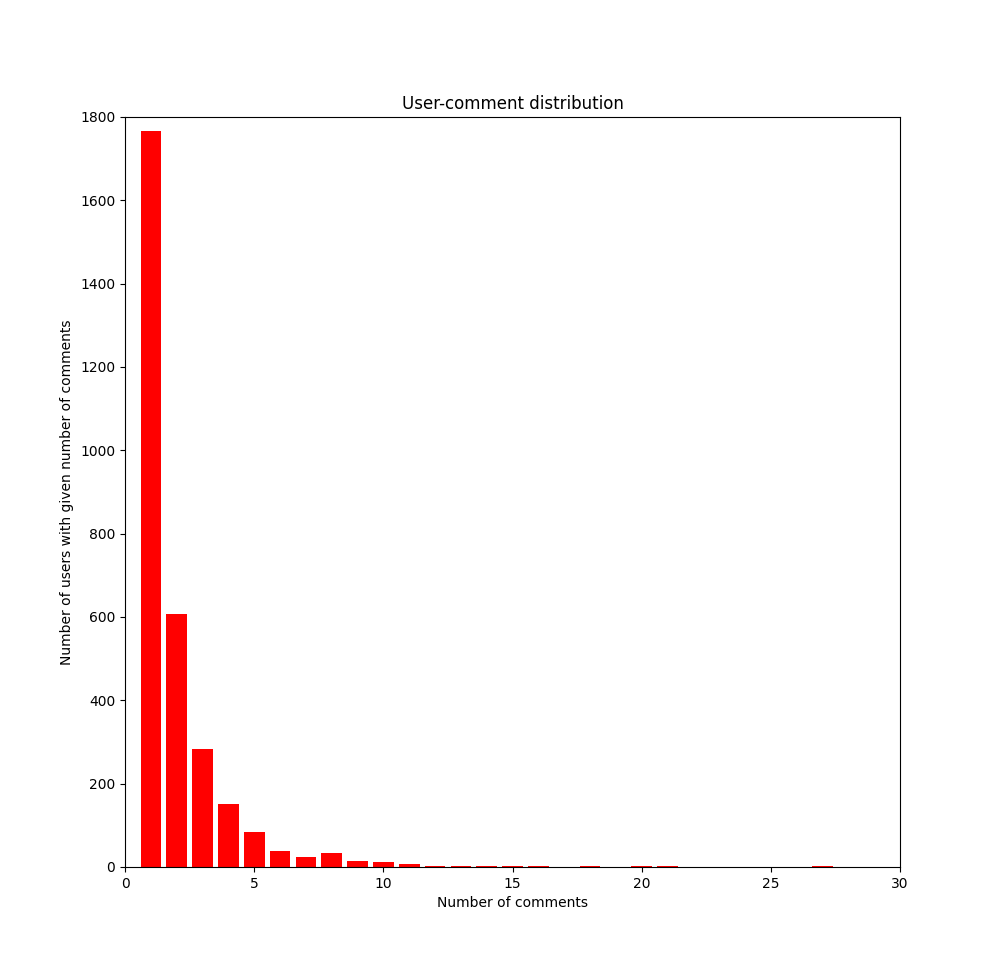
\includegraphics[width=\linewidth]{usercommentdistribution.png}
   \caption{User-Comment Distribution}
  \label{fig:usercomment}
\end{figure}
\textbf{Diagnosed group.} To get textual comments outlining the experiences of MS patients, we will utilize free text data from the MSRegister database \citep{Ford:12}. We chose to use this database because it provides a large, rich resource of experiences of patients diagnosed with MS, in text format. However, one problem of using this dataset directly for our use-case is that the experiences of the patients are recorded post MS diagnosis, which means patients often refer to their condition (that is, multiple sclerosis), in their comments. However, since the classifier will be used pre-diagnosis, we cannot make this classifier rely on the term “multiple sclerosis”, or any other term that only MS patients will know about. Therefore, we remove all clauses containing MS-related terms (footnote with list link) from patient comments. If every clause in a patient comment includes some MS-related term, then we omit the comment from our dataset. With this approach, we were able to get 6121 comments from 3037 diagnosed users in our dataset. \\
\indent \textbf{Control group.} To get the experiences of users who do not have MS (that is, the control group), we chose social media platforms because, like the MSRegister database, people share their experiences in text format on these platforms. Twitter and Reddit were chosen as the social media platforms because they are popular platforms where users often post in plain text about their general life experiences. Therefore, from these social media platforms, we construct two separate control groups. The explanation for the need for two control groups and the description of how these control groups were constructed are outlined below. \\
\indent The first control group constitutes random users from Twitter and Reddit who have not mentioned the term “MS” or any related terms in their timeline. The dataset was constructed such that there is an equal probability for a potential control user to be selected from Twitter or from Reddit. Moreover, we ignored image-only posts, video-only posts, Twitter retweets and Reddit cross-posts. For Reddit, we added the additional restriction that the potential control group user has never posted on any MS-related subreddit (footnote). After identifying the users, we select random posts in their timeline to be included in our dataset. The number of posts we select per user is controlled such that the final user-comment distribution is kept the same as the diagnosed users in the dataset, as illustrated in Figure \ref{fig:usercomment}. Finally, as a measure to prevent posts created by bots to be included in our dataset, no more than 5 duplicate posts were allowed by the same user. \\
\indent This first control group is relevant because a classifier trained using this control group can potentially be used to automatically diagnose a social media user for MS. However, we observed a potential problem: since social media contains a large variety of text data, including news, satire and advertisements, a good classifier will likely learn that all this text data corresponds to a person not having MS. Thus, although a classifier resulting from control one can be used in social media for MS diagnosis, it may still be inaccurate in clinical settings. To solve this problem, we need to create another control group containing experiences of patients diagnosed with another illness. \\
\indent Therefore, the second control group are comments of users who have given self-reported diagnoses of diabetes on social media (both type 1 and type 2), and who, like the first control group, have not mentioned “MS” or any related terms in their timeline. Diabetes was chosen as the illness for the second control group because firstly, it is an incurable, chronic condition like MS, and secondly, it is relatively prevalent, so we can find enough users on social media to exactly match the number of MS-diagnosed users from the MSRegister dataset. The users were found by searching on Twitter and Reddit for high-precision diagnostic patterns (footnote), examples of which can be found in Figure ****. After identifying these users, we only include posts where the user mentions their condition (that is, diabetes), because we would expect only those experiences to be presented to a primary healthcare provider. Then, like what we did for the diagnosed users, we remove all clauses with the word “diabetes” from the text, since the classifier will be used pre-diagnosis, and we cannot make the classifier rely on the term “diabetes” for classifying patients who do not have MS. \\
\indent For both the control groups, the number of comments and the user-comment distribution was kept the same as the diagnosed users. However, the age and gender of the users could not be controlled for since APIs of social media platforms do not provide this data.
\subsection{Ethics and privacy}
The risks associated with our data collection and data access methods are minimal. All the posts collected from Twitter and Reddit were publicly available through the Twitter and Reddit API respectively. We replaced social media usernames with user identifier codes to anonymise their identity. Although the MSRegister database contains identifiable information, including the gender and date of birth of the patients, this database was accessed through a secure virtual desktop environment, so the identifiable information remains private. For both the patients in the MSRegister database and the social media users, we made no attempt identify the users with other external sources of information. Therefore, this research was conducted in compliance to the GDBR guidelines of data protection \citep{GDBR:16}.
\section{Datset Analysis}
\begin{figure*}[h!]
  \centering
  \begin{subfigure}[b]{0.3\linewidth}
    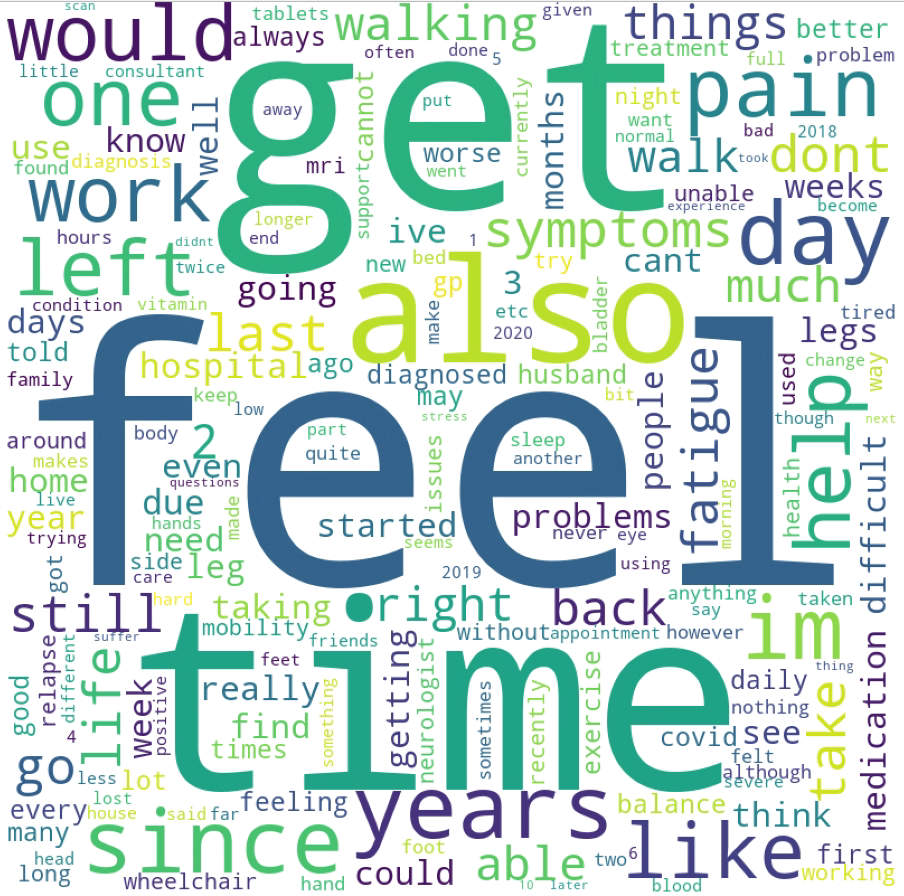
\includegraphics[width=\linewidth]{msregisterfinal.png}
    \caption{Diagnosed Users (MS)}
  \end{subfigure}
  \hspace{1em}
  \begin{subfigure}[b]{0.3\linewidth}
    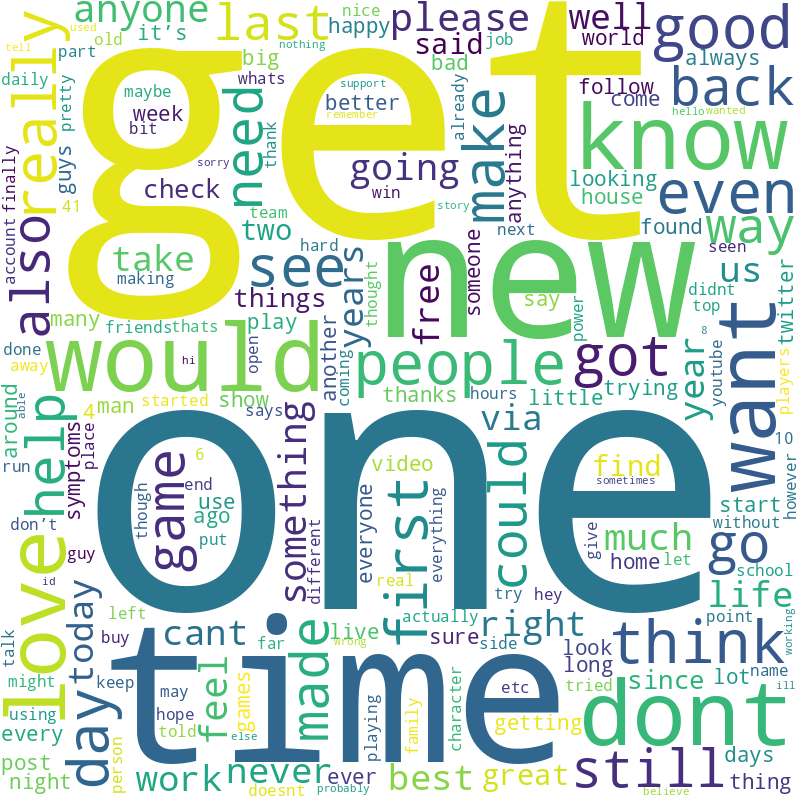
\includegraphics[width=\linewidth]{controlonefinal.png}
    \caption{Control One (Generic)}
  \end{subfigure}
  \hspace{1em}
  \begin{subfigure}[b]{0.3\linewidth}
    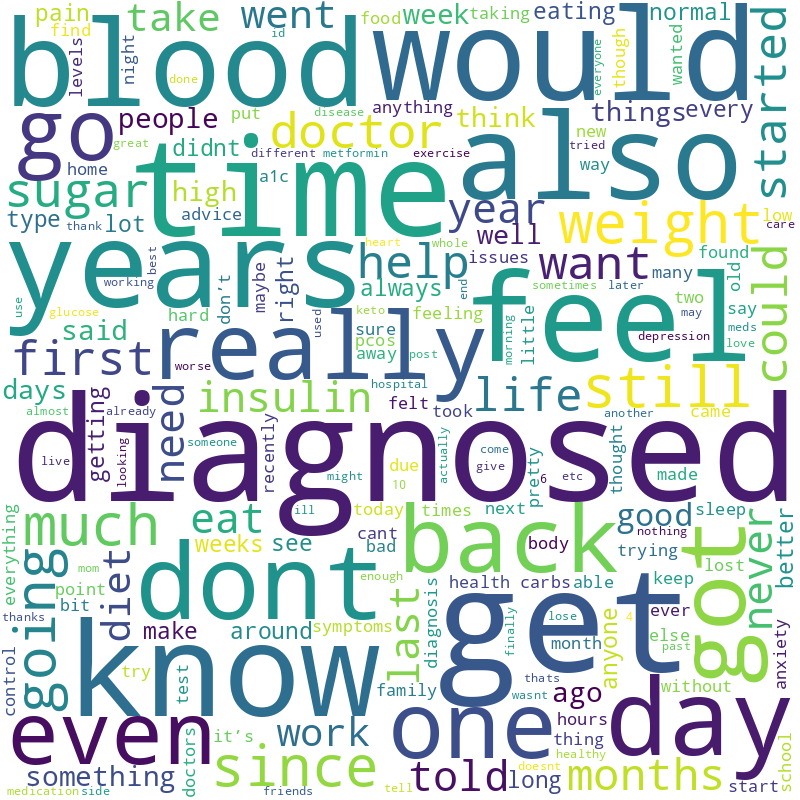
\includegraphics[width=\linewidth]{controltwofinal.png}
    \caption{Control Two (Diabetes)}
  \end{subfigure}
  \caption{Word Clouds For Different Parts Of The Dataset}
  \label{fig:wordclouds}
\end{figure*}
To increase our understanding of the newly created dataset, we started by conducting some preliminary data analysis on our dataset. \\
\indent To begin with, we created word clouds from the text given by the MS-diagnosed users (Figure \ref{fig:wordclouds}a), the generic control one users (Figure \ref{fig:wordclouds}b), and the diabetes control two users (Figure \ref{fig:wordclouds}c).  Before creating each of these word clouds, the text was made lowercase, stop words were removed from the text, and the text was tokenized. \\
\indent Inspecting the word clouds, we see that it is consistent with our expectations of the various parts of the dataset. Words prevalent in the MS-diagnosed group that are absent in the other groups are ‘fatigue’, ‘walking’, ‘pain’, ‘support’ and ‘wheelchair’, which are words representing symptoms of MS \citep{Gustavsen:21}. Common words in the diabetes control group are ‘diet’, ‘weight’, ‘eating’, 'sugar', and 'blood', which is as expected given the symptoms of diabetes \citep{Ramachandran:14}. The generic control group contains common words used in social media, such as ‘love’, ‘game’, ‘people’ and ‘one’. Words used commonly in the English language, like ‘time’ and ‘get’ were present in all three sections of the dataset. Another notable point is that the word ‘ms’ is not present in the MS-diagnosed group and the word ‘diabetes’ is not present in the diabetes control group. This is consistent with the dataset construction method because all clauses with the word ‘ms’ were removed from the MS-diagnosed dataset and similarly all clauses with the word ‘diabetes’ were removed from the diabetes control group, as explained in the ‘Dataset construction’ section above. \\
\indent In addition to generating the word clouds for the dataset, we decided to count the average number of tokens per comment for each part of the dataset. The results of this investigation are shown in Table ****. We observe that the average number of tokens is the greatest for the diabetes control group, lower for the MS-diagnosed control group and lowest for the generic social media control group. Since sentence length varies significantly across the dataset, we need to ensure that the classifiers we train on the dataset do not rely only on the length of the comment for text classification. The implications of this difference are further discussed in the next section.
\begin{table}
\centering
\begin{tabular}{p{0.5\linewidth}p{0.4\linewidth}}
\hline
\textbf{Dataset} & \textbf{Average number of tokens per comment}\\
\hline
Diagnosed (MS) & {29.1} \\
Control One (Generic) & {14.1} \\
Control Two (Diabetes) & {85.3} \\ 
\hline
\end{tabular}
\caption{Average number of tokens per comment for evry part of the dataset}
\label{tab:}
\end{table}
\section{Experiments}
In order to understand which classifier is the best for detecting MS, we experimented several ways to convert text to word vectors and we applied various classification models on these word vectors. \\
\indent However, before conducting any experiments, we pre-processed the dataset as follows. We removed any punctuation and URLs from the free text and made all the characters lowercase. To handle hashtags, tags, and subreddit names in the text collected from social media, we removed the characters ‘\#’, ‘@’ and ‘r/’ from the start of every word in the free text, if the word started with any of those characters. Finally, we tokenized, lemmatized and removed stop words (footnote) from the text in the database. \\
\indent After pre-processing, we explored three ways of converting the pre-processed text into word vectors: bag of words (BoW), tf-idf weighted BoW, and word embeddings. For BoW and tf-idf weighted BoW, the vocabulary was set to 1600. Therefore, the dimension of every word vector was 1600. For word embeddings, we employed word2vec embeddings pretrained using the continuous bag-of-words (CBOW) method on the Google News dataset \citep{Mikolav:13}. The dimension of each of these pretrained word vectors was 300. For each of the classifiers below (except RNN and LSTM), we also average the word embeddings of all the tokens in every comment to get an embedding for each comment. We then use this embedding as input to the model. \\
\indent The dataset was then split into 80\% training dataset and a 20\% testing dataset. For each of the three methods to convert text into word vectors, we train and test the dataset on the following classifiers: \\
\indent \textbf{Logistic Regression.} We started by training a simple logistic regression model on the word vectors. \\
\indent \textbf{Naïve Bayes.} For the BoW vectors and the tf-idf weighted BoW, we train the probabilistic multinomial Naïve Bayes classifier. Since the multinomial Naïve Bayes classifier expects positive word vectors and our word embeddings contain values from -1 to 1, we normalize the word embedding values to the range 0 to 1 and then train the classifier. \\
\indent \textbf{K-Nearest Neighbours (KNN).} For the KNN classifier, we set the value k to 1, 2, 3, 5, 8, 10, and 100. The best accuracy was then recorded in Table ***. \\
\indent \textbf{Neural Network.} We decided to investigate both a single-layer neural network and two-layer neural network. We set the number of epochs to 10 and batch size to 64. In the final layer, we use the sigmoid activation function, and for non-output layers, we tried both the ReLU and tanh activation function. For the two-layer neural network, we set the number of neurons in the hidden layer to 50, 100 and 200. After testing these hyperparameters, the best accuracy was then recorded in Table ****. \\
\indent \textbf{Recurrent Neural Network (RNN).} Since we need an embedding for each word for the RNN, BoW and tfidf-weighted BoW cannot be used for this model. Furthermore, the RNN, by nature of being a sequential model, exemplifies the difference between input sequence lengths. Since we know that the average comment length varies considerably in different sections of the dataset, as shown in Table **** in Section ****, for RNNs we particularly need to make sure that the classifier does not rely only on the length of the text for classification. Therefore, we set the number of RNN units to minimum of the average comment lengths of the datasets in question (rounded up). Accordingly, from the values in Table **** in Section ****, we set the number of RNN units for diagnosed users vs. control one (generic) to be 15 and diagnosed users vs. control two (diabetes) to 30. Then, any comments with longer lengths were truncated to the number of RNN units. This strategy ensures that the classifier relies on the content of the text rather than its length. Lastly, we set the number of epochs to 10 and batch size to 64 before training. \\
\indent \textbf{Long Short-Term Memory Network (LSTM).} The hyperparameters used for the LSTM model were kept the same as the RNN, and for the same reasons as the RNN. BoW and tfidf-weighted BoW could not be used for this model as well, and the number of LSTM units was again chosen to be 15 with control one and 30 with control two. The number of epochs was set to 10 and batch size to 64. \\
\indent The results for each of these classification models are reported in Table ****. \\
****Tables \\
\indent Overall, for control one, word embeddings with a two-layer neural network obtained the best accuracy of 94.3\%. With control two, tf-idf-weighted BoW with a Naïve Bayes classifier had the best accuracy of 92.4\%. We believe that richer, more complicated models like RNNs and LSTMs did not do as well because they must have overfit on the training set, which eventually led to a lower accuracy on the test set. \\
\indent In general, our experiments with control one had higher accuracy than with control two. Therefore, we conclude that classifiers find it easier to distinguish between generic social media text and the experiences of MS patients rather than distinguish between experiences of diabetes patients and MS patients. \\
\indent Another interesting observation is that for control two, word embeddings always performed worse than BoW or tf-idf-weighted BoW, even though word embeddings are usually known for having more semantic richness than BoW models \citep{Mikolav:13}. This result can be explained by the fact that BoW models give more weight to particular words, which likely correspond to symptoms of MS and diabetes in this case. On the other hand, word embeddings cannot distinguish that well between the MS-diagnosed user group and the diabetes control because comments from both these groups contain medical terminology and are thus likely to have similar word embeddings.
\section{Conclusion}
By employing a novel approach combining social media data with the MSRegister dataset of MS patients in the UK, we were able to create the largest ever dataset for computerized diagnosis for MS. We trained multiple different models on this dataset, and we were able to achieve a maximum accuracy of 94.3\% when classifying experiences of MS patients against generic social media text data and a maximum accuracy of 92.4\% against experiences of diabetes patients. This result is significant because with the classifiers trained in this paper, it may be possible to not only detect multiple sclerosis from the patients’ clinical notes, but also from their social media posts. Resulting early diagnosis of MS allows immediate measures to be taken and the symptoms of MS to be controlled. \\
\indent However, we concede that there are still some limitations in our work that can be improved by future research on this topic.  Firstly, there can be further improvements in the construction of the control group of users. With control group two for example, we essentially work with only two diseases – MS and diabetes – which is not like diagnosis in a clinical context, where there are more diseases to account for. In future research therefore, we can have a control group with more illnesses, so the experiments more closely resemble a situation that primary healthcare providers face. In addition, newer, transformer models like BERT and GPT-2 can be applied to this task in future work. While constructing the dataset, although we remove any clause with the term “MS” to prevent the trivial text classification of post-diagnosis comments, we still assume that the experiences of a patient post-diagnosis are the same the same as the experiences of the patient pre-diagnosis. In future work, patients can be asked about their experiences before the diagnosis of MS to create a more reliable dataset for MS diagnosis.
\bibliography{anthology,acl2020}
\bibliographystyle{acl_natbib}
\appendix
% \section{Appendices}
% \label{sec:appendix}
% \section{Supplemental Material}
% \label{sec:supplemental}

\end{document}
